\section*{Einleitung}

Die umgesetzte Architektur der Beispielapplikation ``Roomies'' besteht aus folgenden zwei Haupt-Komponenten:
\begin{itemize}
	\item Eine Shared Codebase mit \emph{barefoot} \cite{Barefoot}
	\item Eine API-Komponente mit \emph{Express.js} \cite{Expressjs}
\end{itemize}

\begin{figure}[ht]
	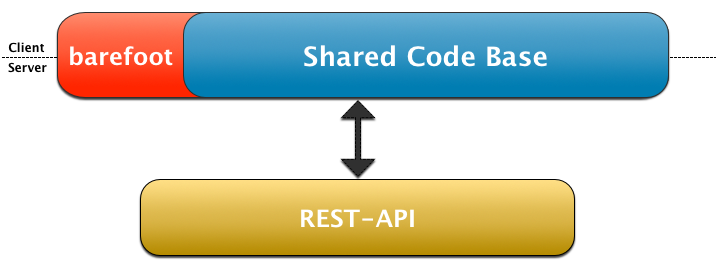
\includegraphics[width=\textwidth]{content/images/grob-layers-sad.png}
	\caption{Übersicht der Architektur}
\end{figure}

\subsection*{Shared Code Base mit barefoot}
Barefoot \cite{Barefoot} ist ein Framework welches während der Bachelorarbeit entwickelt wurde.
Dieses Framework ermöglicht Client und Server den gleichen Code für die MVC-Komponenten zu benutzen und setzt auf
Backbone.js \cite{Backbonejs} auf.

Der Router dient hier als Beispiel:
\begin{lstlisting}[language=JavaScript, caption=Auszug aus Router der Beispielapplikation \cite{roomiesRouter}, label=lst:roomiesRouter, firstnumber=25]
module.exports = Router.extend({
	routes: {
		'': 'home'
		, 'community': 'createCommunity'
		//...
	}

	/** Function: home
	 * Home page which renders the login button if not authorized.
	 * Otherwise it redirects to community/create or community/:slug/tasks.
	 */
	, home: function home() {
		if(!this.isAuthorized()) {
			this.render(this.createView(HomeView));
		} else {
			var community = this.dataStore.get('community');
			if(!community) {
				this.navigate('community/create', { trigger: true });
			} else {
				this.navigate('community/' + community.get('slug') +
					'/tasks', { trigger: true });
			}
		}
	}

	/** Function: createCommunity
	 * Create community view
	 */
	, createCommunity: function createCommunity() {
		debug('create community');
		if(!this.redirectIfNotAuthorized()) {
			this.render(this.createView(CreateCommunityView));
		}
	}
	//...
});
\end{lstlisting}

Der Router aus Quelltext \ref{lst:roomiesRouter} wird sowohl vom Client als auch vom Server verwendet und registriert URLs mit den entsprechenden Funktionen.

Die ``HomeView'' ist in Quelltext \ref{lst:roomiesHomeView} zu sehen.

\begin{lstlisting}[language=JavaScript, caption=Ausschnitt aus HomeView der Beispielapplikation \cite{roomiesHomeView}, label=lst:roomiesHomeView, firstnumber=7]
module.exports = View.extend({
	el: '#main'
	, template: templates.login

	/** Function: renderView
	 * Renders the home view.
	 */
	, renderView: function renderView() {
		this.$el.html(this.template({}));
	}

	/** Function: afterRender
	 * Sets the document title.
	 */
	, afterRender: function afterRender(resolve) {
		var _super = this.constructor.__super__.afterRender.bind(this);

		this.setDocumentTitle(this.translate('Welcome'));
		_super(resolve);
	}
	//...
});
\end{lstlisting}

\subsection*{API-Komponente}
Auf Server-Seite ist eine REST-API \cite{REST} erstellt worden. Die Shared Codebase greift auf diese zu, um Daten zu speichern oder zu laden.

Dabei unterscheidet ``barefoot'' intelligent zwischen API-Aufrufen des Servers oder des Clients.
Ruft der Client eine API auf, wird ein AJAX-Aufruf gemacht. Wird die API
hingegen vom Server aus aufgerufen, werden direkt die entsprechend definierten
Callbacks für die gewünschte Route lokal aufgerufen.

Quelltext \ref{lst:roomiesControllerExample} zeigt ein Beispiel für einen solchen
Callback, während Quelltext \ref{lst:roomiesComponentExample} ein Beispiel für
eine API-Route aufzeigt.

\begin{lstlisting}[language=JavaScript, caption=API-Controller Beispiel \cite{roomiesCommunityApiExample}, label=lst:roomiesControllerExample, firstnumber=294]
/** Function: getCommunityWithId
 * Looks up a community with a specific ID.
 *
 * Parameters:
 *   (Function) success - Callback on success. Will pass the community data
 *                        as first argument.
 *   (Function) error - Callback in case of an error
 *   (String) id - The id of the community to look for.
 */
function getCommunityWithId(success, error, id) {
	debug('get community with id');

	var communityDao = getCommunityDao.call(this)

		/* AnonymousFunction: forwardError
		 * Forwards an error object using the error callback argument
		 */
		, forwardError = function forwardError(err) {
			return error(err);
		}

		/* AnonymousFunction: afterCommunitySearch
		 * Calls the success or error callback after searching for a community.
		 */
		, afterCommunitySearch = function afterCommunitySearch(community) {
			if(!_.isNull(community)) {
				success(community.dataValues);
			} else {
				forwardError(new errors.NotFoundError(
					'Community with id ' + id + 'does not exist.')
				);
			}
		};

	communityDao.find({ where: { id: id, enabled: true }})
		.success(afterCommunitySearch)
		.error(forwardError);
}
\end{lstlisting}

\begin{lstlisting}[language=JavaScript, caption=API-Route Beispiel \cite{communityApiDefinition}, label=lst:roomiesComponentExample, firstnumber=31]
var prefix = apiPrefix + modulePrefix;

// GET /api/community/:id
api.get(prefix + '/:id(\\d+)', [
	basicAuthentication
	, authorizedForCommunity
	, controller.getCommunityWithId]);
\end{lstlisting}

Die Beispielapplikation ist somit nach dem MVC-Pattern aufgebaut. \\
Die einzelnen Komponenten haben folgende Aufgabe:
\begin{itemize}
	\item{\textbf{M}odel ist ein traditionelles Model welches zwischen Server \& Client geteilt wird}
	\item{\textbf{V}iew ist eine ``Barefoot.View'' \cite{BarefootView} und rendert Templates}
	\item{\textbf{C}ontroller ist einerseits ein ``Route''-Controller, welcher aufgrund von URLs die richtige View aufruft und andererseits ein API-Controller, welcher die REST-API-Logik kapselt}
\end{itemize}

\newpage
Diagramm \ref{fig:mvcComponentDiagramm} zeigt eine grobe Übersicht über das Zusammenspiel der verschiedenen Komponenten.

\begin{figure}[ht!]
	\centering{
		% Graphic for TeX using PGF
% Title: /Users/michael/code/BA/dokumentation/content/sad/diagrams/mvc-components.dia
% Creator: Dia v0.97.2
% CreationDate: Tue Jun 11 13:04:15 2013
% For: michael
% \usepackage{tikz}
% The following commands are not supported in PSTricks at present
% We define them conditionally, so when they are implemented,
% this pgf file will use them.
\ifx\du\undefined
  \newlength{\du}
\fi
\setlength{\du}{15\unitlength}
\begin{tikzpicture}
\pgftransformxscale{1.000000}
\pgftransformyscale{-1.000000}
\definecolor{dialinecolor}{rgb}{0.000000, 0.000000, 0.000000}
\pgfsetstrokecolor{dialinecolor}
\definecolor{dialinecolor}{rgb}{1.000000, 1.000000, 1.000000}
\pgfsetfillcolor{dialinecolor}
\pgfsetlinewidth{0.100000\du}
\pgfsetdash{}{0pt}
\definecolor{dialinecolor}{rgb}{1.000000, 1.000000, 1.000000}
\pgfsetfillcolor{dialinecolor}
\fill (16.000000\du,3.000000\du)--(16.000000\du,10.000000\du)--(29.000000\du,10.000000\du)--(29.000000\du,3.000000\du)--cycle;
\definecolor{dialinecolor}{rgb}{0.000000, 0.000000, 0.000000}
\pgfsetstrokecolor{dialinecolor}
\draw (16.000000\du,3.000000\du)--(16.000000\du,10.000000\du)--(29.000000\du,10.000000\du)--(29.000000\du,3.000000\du)--cycle;
\definecolor{dialinecolor}{rgb}{1.000000, 1.000000, 1.000000}
\pgfsetfillcolor{dialinecolor}
\fill (16.000000\du,2.000000\du)--(16.000000\du,3.000000\du)--(18.510000\du,3.000000\du)--(18.510000\du,2.000000\du)--cycle;
\definecolor{dialinecolor}{rgb}{0.000000, 0.000000, 0.000000}
\pgfsetstrokecolor{dialinecolor}
\draw (16.000000\du,2.000000\du)--(16.000000\du,3.000000\du)--(18.510000\du,3.000000\du)--(18.510000\du,2.000000\du)--cycle;
% setfont left to latex
\definecolor{dialinecolor}{rgb}{0.000000, 0.000000, 0.000000}
\pgfsetstrokecolor{dialinecolor}
\node[anchor=west] at (16.000000\du,2.500000\du){Server};
\pgfsetlinewidth{0.100000\du}
\pgfsetdash{}{0pt}
\definecolor{dialinecolor}{rgb}{1.000000, 1.000000, 1.000000}
\pgfsetfillcolor{dialinecolor}
\fill (13.000000\du,13.000000\du)--(13.000000\du,23.000000\du)--(32.000000\du,23.000000\du)--(32.000000\du,13.000000\du)--cycle;
\definecolor{dialinecolor}{rgb}{0.000000, 0.000000, 0.000000}
\pgfsetstrokecolor{dialinecolor}
\draw (13.000000\du,13.000000\du)--(13.000000\du,23.000000\du)--(32.000000\du,23.000000\du)--(32.000000\du,13.000000\du)--cycle;
\definecolor{dialinecolor}{rgb}{1.000000, 1.000000, 1.000000}
\pgfsetfillcolor{dialinecolor}
\fill (13.000000\du,12.000000\du)--(13.000000\du,13.000000\du)--(15.510000\du,13.000000\du)--(15.510000\du,12.000000\du)--cycle;
\definecolor{dialinecolor}{rgb}{0.000000, 0.000000, 0.000000}
\pgfsetstrokecolor{dialinecolor}
\draw (13.000000\du,12.000000\du)--(13.000000\du,13.000000\du)--(15.510000\du,13.000000\du)--(15.510000\du,12.000000\du)--cycle;
% setfont left to latex
\definecolor{dialinecolor}{rgb}{0.000000, 0.000000, 0.000000}
\pgfsetstrokecolor{dialinecolor}
\node[anchor=west] at (12.900000\du,12.500000\du){Shared};
\pgfsetlinewidth{0.100000\du}
\pgfsetdash{}{0pt}
\definecolor{dialinecolor}{rgb}{1.000000, 1.000000, 1.000000}
\pgfsetfillcolor{dialinecolor}
\fill (20.000000\du,15.000000\du)--(20.000000\du,16.400000\du)--(25.022500\du,16.400000\du)--(25.022500\du,15.000000\du)--cycle;
\definecolor{dialinecolor}{rgb}{0.000000, 0.000000, 0.000000}
\pgfsetstrokecolor{dialinecolor}
\draw (20.000000\du,15.000000\du)--(20.000000\du,16.400000\du)--(25.022500\du,16.400000\du)--(25.022500\du,15.000000\du)--cycle;
% setfont left to latex
\definecolor{dialinecolor}{rgb}{0.000000, 0.000000, 0.000000}
\pgfsetstrokecolor{dialinecolor}
\node at (22.511250\du,15.750000\du){Controller};
\pgfsetlinewidth{0.100000\du}
\pgfsetdash{}{0pt}
\definecolor{dialinecolor}{rgb}{1.000000, 1.000000, 1.000000}
\pgfsetfillcolor{dialinecolor}
\fill (19.300000\du,5.900000\du)--(19.300000\du,7.300000\du)--(25.790000\du,7.300000\du)--(25.790000\du,5.900000\du)--cycle;
\definecolor{dialinecolor}{rgb}{0.000000, 0.000000, 0.000000}
\pgfsetstrokecolor{dialinecolor}
\draw (19.300000\du,5.900000\du)--(19.300000\du,7.300000\du)--(25.790000\du,7.300000\du)--(25.790000\du,5.900000\du)--cycle;
% setfont left to latex
\definecolor{dialinecolor}{rgb}{0.000000, 0.000000, 0.000000}
\pgfsetstrokecolor{dialinecolor}
\node at (22.545000\du,6.700000\du){ApiController};
\pgfsetlinewidth{0.100000\du}
\pgfsetdash{}{0pt}
\definecolor{dialinecolor}{rgb}{1.000000, 1.000000, 1.000000}
\pgfsetfillcolor{dialinecolor}
\fill (15.000000\du,19.000000\du)--(15.000000\du,20.400000\du)--(17.662500\du,20.400000\du)--(17.662500\du,19.000000\du)--cycle;
\definecolor{dialinecolor}{rgb}{0.000000, 0.000000, 0.000000}
\pgfsetstrokecolor{dialinecolor}
\draw (15.000000\du,19.000000\du)--(15.000000\du,20.400000\du)--(17.662500\du,20.400000\du)--(17.662500\du,19.000000\du)--cycle;
% setfont left to latex
\definecolor{dialinecolor}{rgb}{0.000000, 0.000000, 0.000000}
\pgfsetstrokecolor{dialinecolor}
\node at (16.331250\du,19.750000\du){View};
\pgfsetlinewidth{0.100000\du}
\pgfsetdash{}{0pt}
\definecolor{dialinecolor}{rgb}{1.000000, 1.000000, 1.000000}
\pgfsetfillcolor{dialinecolor}
\fill (27.000000\du,19.000000\du)--(27.000000\du,20.400000\du)--(30.235000\du,20.400000\du)--(30.235000\du,19.000000\du)--cycle;
\definecolor{dialinecolor}{rgb}{0.000000, 0.000000, 0.000000}
\pgfsetstrokecolor{dialinecolor}
\draw (27.000000\du,19.000000\du)--(27.000000\du,20.400000\du)--(30.235000\du,20.400000\du)--(30.235000\du,19.000000\du)--cycle;
% setfont left to latex
\definecolor{dialinecolor}{rgb}{0.000000, 0.000000, 0.000000}
\pgfsetstrokecolor{dialinecolor}
\node at (28.617500\du,19.750000\du){Model};
\pgfsetlinewidth{0.100000\du}
\pgfsetdash{{1.000000\du}{1.000000\du}}{0\du}
\pgfsetdash{{0.300000\du}{0.300000\du}}{0\du}
\pgfsetmiterjoin
\pgfsetbuttcap
{
\definecolor{dialinecolor}{rgb}{0.000000, 0.000000, 0.000000}
\pgfsetfillcolor{dialinecolor}
% was here!!!
\pgfsetarrowsend{stealth}
{\pgfsetcornersarced{\pgfpoint{0.000000\du}{0.000000\du}}\definecolor{dialinecolor}{rgb}{0.000000, 0.000000, 0.000000}
\pgfsetstrokecolor{dialinecolor}
\draw (16.331250\du,19.000000\du)--(16.331250\du,15.700000\du)--(20.000000\du,15.700000\du);
}}
\pgfsetlinewidth{0.100000\du}
\pgfsetdash{}{0pt}
\pgfsetdash{}{0pt}
\pgfsetbuttcap
{
\definecolor{dialinecolor}{rgb}{0.000000, 0.000000, 0.000000}
\pgfsetfillcolor{dialinecolor}
% was here!!!
\pgfsetarrowsend{stealth}
\definecolor{dialinecolor}{rgb}{0.000000, 0.000000, 0.000000}
\pgfsetstrokecolor{dialinecolor}
\draw (20.000000\du,16.400000\du)--(17.662500\du,19.000000\du);
}
\pgfsetlinewidth{0.100000\du}
\pgfsetdash{{1.000000\du}{1.000000\du}}{0\du}
\pgfsetdash{{0.300000\du}{0.300000\du}}{0\du}
\pgfsetbuttcap
{
\definecolor{dialinecolor}{rgb}{0.000000, 0.000000, 0.000000}
\pgfsetfillcolor{dialinecolor}
% was here!!!
\pgfsetarrowsend{stealth}
\definecolor{dialinecolor}{rgb}{0.000000, 0.000000, 0.000000}
\pgfsetstrokecolor{dialinecolor}
\draw (26.950580\du,19.700000\du)--(17.662500\du,19.700000\du);
}
\pgfsetlinewidth{0.100000\du}
\pgfsetdash{}{0pt}
\pgfsetdash{}{0pt}
\pgfsetbuttcap
{
\definecolor{dialinecolor}{rgb}{0.000000, 0.000000, 0.000000}
\pgfsetfillcolor{dialinecolor}
% was here!!!
\pgfsetarrowsend{stealth}
\definecolor{dialinecolor}{rgb}{0.000000, 0.000000, 0.000000}
\pgfsetstrokecolor{dialinecolor}
\draw (17.662500\du,20.400000\du)--(27.000000\du,20.400000\du);
}
\pgfsetlinewidth{0.100000\du}
\pgfsetdash{}{0pt}
\pgfsetdash{}{0pt}
\pgfsetbuttcap
{
\definecolor{dialinecolor}{rgb}{0.000000, 0.000000, 0.000000}
\pgfsetfillcolor{dialinecolor}
% was here!!!
\pgfsetarrowsend{stealth}
\definecolor{dialinecolor}{rgb}{0.000000, 0.000000, 0.000000}
\pgfsetstrokecolor{dialinecolor}
\draw (25.022500\du,16.400000\du)--(27.000000\du,19.000000\du);
}
\pgfsetlinewidth{0.100000\du}
\pgfsetdash{}{0pt}
\pgfsetdash{}{0pt}
\pgfsetmiterjoin
\pgfsetbuttcap
{
\definecolor{dialinecolor}{rgb}{0.000000, 0.000000, 0.000000}
\pgfsetfillcolor{dialinecolor}
% was here!!!
\pgfsetarrowsend{stealth}
{\pgfsetcornersarced{\pgfpoint{0.000000\du}{0.000000\du}}\definecolor{dialinecolor}{rgb}{0.000000, 0.000000, 0.000000}
\pgfsetstrokecolor{dialinecolor}
\draw (22.545000\du,7.300000\du)--(22.545000\du,11.000000\du)--(28.617500\du,11.000000\du)--(28.617500\du,19.000000\du);
}}
\pgfsetlinewidth{0.100000\du}
\pgfsetdash{{1.000000\du}{1.000000\du}}{0\du}
\pgfsetdash{{0.300000\du}{0.300000\du}}{0\du}
\pgfsetmiterjoin
\pgfsetbuttcap
{
\definecolor{dialinecolor}{rgb}{0.000000, 0.000000, 0.000000}
\pgfsetfillcolor{dialinecolor}
% was here!!!
\pgfsetarrowsend{stealth}
{\pgfsetcornersarced{\pgfpoint{0.000000\du}{0.000000\du}}\definecolor{dialinecolor}{rgb}{0.000000, 0.000000, 0.000000}
\pgfsetstrokecolor{dialinecolor}
\draw (30.235000\du,19.000000\du)--(30.235000\du,6.600000\du)--(25.790000\du,6.600000\du);
}}
\end{tikzpicture}

	}

	\caption{MVC-Komponenten im Zusammenspiel}
	\label{fig:mvcComponentDiagramm}
\end{figure}